% Chapters
\documentclass[12pt]{book}
\usepackage{graphicx}
\usepackage[a4paper,margin=4cm]{geometry}
\usepackage{natbib}
\usepackage{caption}
\begin{document}
\chapter[State of the art]{Electricity markets and complexity: State of the art}
\label{Chapter1} % Change X to a consecutive number; for referencing this chapter elsewhere, use 
\ref{Chapter1}
%---------------------------------------------------------------------------------------%	
SECTION 1
%----------------------------------------------------------------------------------------
 
\section{Introduction}
The electricity markets have undergone a transformation in recent years, under the pretense of operating in more competitive and profitable environments. Thus in many economies around the world it has gone from big monopolies to oligopolies, where competition laws of supply and demand govern their behavior \cite{krause2006}.

On the other hand the experience of the agents involved in these kind of markets are increasingly, their level of knowledge of the environment, and the facility for access to information, making the competition more dynamic. Thus, more robust models for measuring risk are required, allowing them to implement the planning of the operation in the short and medium term.

Each agent has defined objectives, in most cases profit maximization under different constraints of internal or external character \cite{gnansounou2004}. In this type of scenarios with open markets and free competition, it is a very complex consideration of all the variables involved, however from different methodologies can be approximations to the physical phenomena that happens.

One of the biggest complications is the exercise of predict the demand, which is a critical variable for generating prices. To this end there are plenty of models with the aim of establishing the best strategy in the energy auctions, which optimizes the profitability of generators but excludes income from traders whose main function is brokering with a different risk exposure.

On the other side, with the aim of ensuring compliance of the transactions, there are no mechanisms to assess the interaction of financial performance between traders of coordinated manner \cite{zhou2007}. This process is delegated to free market movement, and is done partially or by studying the individual situation of each agent, through indicators that not reflects the dynamics of interactions.

In that sense, the need for models to measure the performance of financial affairs for the traders and generators is obvious. These models will be oriented to the interaction between participants, their complexity and severity if a difficulty appears. Thus, each participant take forward a strategy to maximize their returns, which is displayed as a part of the system elements of the electricity market.

It should be noted that in any market where commercial transactions take place, regardless of the goods or services, uncertainty appears with external and internal nature, like economical, operational and financial, among others. This uncertainty will cause problems that affect the stability of the markets if management and control tools are not used.

\section{Previous studies} Studies about electricity markets and their evolution have been directed towards two major flows. First, the tendency to estimate the market variables such as stock price, the price of contracts, demand level, supply level, generation capacity, among others; by using statistical tools, mathematical formulation or even simulation. Second calculating exhibits in the functional systems, in order to establish with some certainty, the magnitude of the problems that fall within the operation.

In the results found by \cite{tushar2013} the equilibrium between supply and demand through the use of game theory, where consumers play an important role in creating price, was the most important advance. However, to maximize the profitability of the consumer is an ambiguous result, because despite being located at the end of the energy cycle, what which seeks user is the reduction in the cost without generating returns through speculation or even arbitrage, and commonly is not the purpose of the business, it means the consumers used the energy as the necessary good but not like profitable \cite{borenstein1999}.

For his part \cite{medina2007}\cite{sweeting2007}\cite{wolfram1999} worked in the decomposition of the variables involved in process of creating prices, including phenomena such as social affairs, climatic, economic indicators, regulatory requirements, and others, using mathematical techniques, statistics or new technologies, like artificial intelligence. Such decomposition aims at a certain level of confiability, projecting price developments in the future. However one of the major problems that has any model, independent of the methodology used, is the evidence of the ``back testing" results, which commonly diverge of the observed reality.

In the same way, portfolio optimization tools are applied in the generation of electricity \cite{stoft2002} and have gained importance in recent years, allowing producers, maximize their profits considering the main sources of generation. In Colombia hydroelectric generation considers almost 70.35\% of total capacity \cite{sandoval2004} leaving clear evidence of the exposure to climate phenomena. Thus, generation using alternative sources like solar, thermal or wind, have been winning gradually participation in the generation portfolio, which allows having alternatives to ensure supply, based on the recommendations from optimization techniques for energy portfolios.

Continuing with the description, studies as developed by \cite{apt2004} have been trying to visualize the operational phenomenon from the manifestation of blackouts that directly affect energy supply, with the respective economic implications of a country. In recent results achieved by \cite{apt2004} it can determine the possibility of incurring losses due to the materialization of operational events, such as impairment of physical transmission network, system failures, maintenance, changes in voltage, levels of risks, human errors, weather events, among others.

Quantify risk exposures related to the operation, and financial exposures linked to power generation have captured the focus of the different works developed so far \cite{apt2004}\cite{medina2007}\cite{nanduri2009}. While the ideal scenario is that the market remains in equilibrium, where agents maximizes their returns with minimal transaction costs, and where the energy supply is reached without incurring losses. But, there is another factor concerning the adequate capacity to meet contractual obligations, that is, if indeed the agent that has commitments has at the same time the financial strength to honor them.

In this context, research has addressed the problem of interactions between agents from a purely functional or operational perspective. For \cite{apt2004}\cite{medina2007} it is evident that each agent, trader, generator or consumer should established the relationship level with other participants, looking for maximize the results amid the laws of supply and demand, but the control of the financial exposure is another factor which ensures the functionality of the system.

The approach using game theory, has found results through the integration of the decisions of the agents \cite{wiszniewska2008}. Also, agent-based modeling - ABM - aims to explain the phenomenon of interaction in order to engage in proper planning to ensure the satisfaction of the demand \cite{weidlich2008}. And again the problem considers only the functional perspective and the financial stability it is implicitly considered, like an assumption, which always is fulfilled.

About the research, the results from modeling by using ABM can determine the evolution of energy prices based on direct or indirect relations \cite{lebaron2005}, simulate the dynamics to estimate the optimal energy production \cite{young2014} to establish the best alternative for negotiation, considering theorems such as market power \cite{krause2006}\cite{lebaron2005} or even contribute in the management of Smart Grids \cite{apt2004} consolidating information from each participant, with the corresponding impact in the system. However, these studies again obey to the operational performance of the market, and the possibility of explaining the operating phenomenon that happens.

Having said this, it is increasingly evident the need to treat the physical phenomenon from a financial point of view among the participants. Historically, some events of unmet demand have occurred because some agents faced problems in its financial position to honor contractual obligations, even though the reaction is immediate by the regulator \cite{Congreso2013}. If there are presence of weakness in finance accounts, is presented the materialization of risks, where commitments (covenants) can't be honored without the operator of the system can anticipate objectively the occurrence of any event of default, considering the financial information provided by agents and the transactions in the market.

Thus, the construction of an integrated model that determines the positions of financial risk of each agent, with their implications for the market is justified from the point of view of securing the energy supply and more specifically the assurance of the financial equilibrium which means the confiability of the market business.

And the business of electricity has additional particularities, because one of the major premises of the power market, is that demand has a passive position and the offer has an actively position \cite{hurtado2006}\cite{medina2007}. The last affirmation, shall be deemed through the process of construction of the models, because given the integration of the risks and the passivity of the demand, this can't be managed with existences, it means the agent can't store electricity like any merchandise. That?s why working capital and liquidity have particular forms of treatment according to the risk financial measure.

In profitability terms, corporate profits are subject to the submission of tenders firm power and therefore the second step for participants, is to present in detail its financial capacity and that of the other actors involved to make transactions without compromising business viability.

\section{Modeling of energy markets} A market dominated by a small number of service providers or producers of products, is an oligopoly \cite{tremblay2011}, and there are limitations involved with each participant, even if each knows the actions of their competitors in order to preserve the functionality of the market. Similarly if one of the participants changes the conditions of operation, the others must find out instantly because their returns are affected, decreasing competition from all the system. In other words if a participant changes the rules, the others must react immediately. 

In this context the energy markets are oligopoly because participants often pursue strategies, and adapted those strategies in order to change the market conditions \cite{borenstein1999} \cite{stoft2002}. Also, the participants perform approaches, which enable the functionality of operating models in a complex frame, considering the large number of variables and situations to consider \cite{borenstein1999} \cite{yousefi2011}, because they need simulate the different scenarios.

Game theory can represent strategic behavior, however, many of these models are very simple and do not capture the complexity arising from the markets, despite the fact that they brings partial signals of this behavior \cite{stoft2002}. But after all findings and developments from this methodology, we can integrate Game theory with other areas of knowledge in order to improve results.

On the other hand, the agent based model - ABM - overcomes some of the weaknesses of the model of market equilibrium centralized which represents the price formation, and the balance between the competitors ensuring the stability of the system \cite{gnansounou2004}. where the main objective is the fulfillment of the demand but finally not ensure the financial viability of participants. 

AABM models can represent heterogeneous individual agents and their behavior, the rules of the market and the agent?s actions in a decentralized manner (without central control). These models are increasingly used to analyze the decisions made by the generators, distributors, traders, regulators and consumers in a liberalized market \cite{zhou2007}.

In \cite{weidlich2008} iit is done a critical review of the ABM models for electricity markets and they found that most of the models focus on issues of market power and tend to ignore the restrictions of transfers in certain markets. 
The results found in \cite{yu2010} propose the creation of a right in order to obtain profits in congestion scenarios in transmission networks, which allow the recognition of existence of over costs in a congested network, i.e. a solution of an operational common problem. 

However, this proposal acts like the response to an inherent characteristic to the operative system, and again evades the financial relationship between the generator and marketer or even the interactions that consider the methodologies ABM and Game Theory, but from a general perspective.

The models often ignore the market demand answers, the implied characteristics in the evolution of prices and restrictions intervals in the network \cite{medina2007}, and incidentally consider that some assumptions are always fulfilled, like the financial stability. The development of a model ABM, which includes the behavior of demand, price and availability, will allow progress in understanding how the energy markets operate and at the same time the interaction with new technologies and other factors underlying in the market.

The construction of energy market models has focused on the estimation of price developments, forecast of demand, simulation of market strategies from producers agents, defining energy policies, technology selection, among others  \cite{medina2007}. However exploring the interrelationships of the agents with the operation of the electrical system in the short and medium term from the point of view of its financial strength, it is something that should be explored.

And it is important because the properties of an energy market, includes immediate delivery, storage limitations, the inelasticity of the demand in the short term and the fulfillment with the regulation, which allows an agent based modeling - ABM. This methodology is a good approach to understanding the complexity of the system \cite{pakes2015}, but should be treated in depth with the inclusion of interactions between participants and their level of exposure to financial risk, by the way, creating a space for research.

The most important aspect of this research project is the existence of conceptual gaps in the process of modeling electricity markets, related to corporate risk approach. Financial risk factors such as credit risk; counterparty, operational and market can affect the competitive position of the decisions of the agents and impacting the stability of the electricity market.
 
Considerations as macroeconomic issues, financial and solvency type are elements that affect the performance of the agents, their market share and generate administrative actions by the system operator.

It is possible wondering about how to measure the vulnerability of the system agents in front of financial risk factors and how it affects the operation of the market as a whole. Since for such eventualities, there may be episodes of unmet demand, which leads a high opportunity cost, and in the other hand the impact suffered by the national economy that aims to make of opening to global markets a boost to economic growth.

\section{Space research in electricity markets}The market organization and composition of the entities responsible for its administration and operation, is based on agents, which are, generators, transporters, traders, distributors and consumers. This entails that the interaction between them have certain levels of complexity, even more when they exchanges cash flows between them. This specific financial complexity, has not been tested in studies developed by \cite{borenstein1999}\cite{medina2007}\cite{stoft2002}\cite{sweeting2007}\cite{weidlich2008}\cite{wiszniewska2008}, given that the models implemented so far are concentrated in the estimation of energy prices, the modeling of demand levels, the prediction of strategies followed by generator agents, identifying best practices in energy policies, the simulation of supply failures, and even the severity of operational risks.

This does not incorporate the peculiarities of system around the financial and economic interaction of the agents in charge of buying and selling energy to ensure the supply, which is why this research project is relevant and pertinent.

In other words, in many investigations aimed at electricity markets \cite{gnansounou2004}\cite{stoft2002} the results do not consider the possibility that a trader or generator presented problems of liquidity or solvency with highly likely to materialize their counterparty risks, which affects the creation of the price and the market stability because the supply is compromised.

At the same time, energy demand should be reached despite the conditions of the system, for this reason the concentration of research efforts will be directed at ensuring the functioning of the market from all perspectives, allowing anticipate the materialization of operational risk, strategic risk, legal risk, market risk, technological exposition, financial risk, and the proper system operation. Finally considering this research project, the inclusion of financial component.

In that sense, the advances in \cite{apt2004}\cite{sweeting2007}\cite{young2014} have helped to achieve results of operational, strategic, technological type and even in markets functionality, however there is an analytical gap in studies when the financial component is an assumption that input always true, and is fulfilled in all cases. The problem is because one of the assumptions for finding results is the economic and financial feasibility of the agents and as is well known, the financial component depends on a lot of difficult elements to integrate and not always is satisfied in the real operation.

\section{Colombian electricity market: review} The Colombian state, to the early 90's made a detailed review of the management and the energy sector achievements reached in several years of operation. The results were very unfavorable because the participants companies, they found many irregularities in terms of operational, administrative and financial efficiency; even in the results highlight the declaration of insolvency of some of them. The above process triggered the period of national rationing, and it was forced between 1991-1992.

It was necessary to consider the modernization of the electricity sector in Colombia. In this way, making adjustments in line with the scheme implemented in the UK and other countries with similar patterns of operation in energy markets, the country proceeded to the restructuring. Similarly, the 1991 Constitution was signed in order to ensure the provision of efficient public services over the head of the state, in scenarios of competence and quality of the operation. Then it presented the opportunity to integrate these two currents demanding improved conditions of the energy market, i.e. quality and competence.

The New Constitution designates the state's obligation to provide the public services, allowing the main achievement regarding the creation and definition of standards for the maintenance of the entities responsible for the regulation, administration, planning and control of the market. Private companies could provide public services, but the state would make the tasks of regulation and control of the operation \cite{Aguilar2004}.

Article 365. \textit{Public services are inherent to the social purpose of the State. The State should ensure its efficient delivery to all inhabitants of the country} \cite{de1991}.

Public services are subject to the legal regime established by law, they may be provided by the State, directly or indirectly, by organized communities or individuals. In any case, the State shall maintain the regulation, control and monitoring of these services \cite{Aguilar2004}.

If for reasons of sovereignty or social interest, the State, by law approved by a majority of the members of each chamber, initiated by the Government decides to reserve certain strategic activities or public services must compensate prior and fully to people under that law, deprived of the exercise of a lawful activity \cite{Aguilar2004}.

By Decree 2119 of 1992, the former national commission of energy was transformed in ``Unidad de planeaci\'on minero energ\'etica" (UPME); he reformed the Ministry of Mines and Energy, and the Energy Regulatory Commission, which is under the Ministry of mines and Energy. The latter commission was created with the aim of advancing the regulatory activities of the energy sector, which includes the price adjustments necessary for equitable service delivery, but forgot the financial sustainability.

In 1994, the state promulgated the laws 142 (known as the Public Services Law) and 143 (Electricity Act), for the design and subsequent consolidation of an effective institutional structure, which supports the requirements of the utilities sector. Thus sought to achieve goals in the face of social and economic sustainability, embodied in the constitution \cite{Aguilar2004}, and again the law mentioned the finality but not the assumptions as a competitive financial structure.

The new regulatory framework, created the ``Mercado de Energ\'ia Mayorista" (MEM), which is monitored by the ``Comisi\'on de regulaci\'on de Energ\'ia y Gas"  (CREG). The objective of MEM was the organization of each of the participants about the transactions of buying and selling energy, providing a stage of free competition. 

Another characteristic of MEM was the categorization of energy contracts between generators and traders as financial assets, so that it could establish the surpluses or shortages resulting from transactions, also achieving the quantification of losses and profits versus actual demand, leaving the interactions as a problem of the market.

Some of the functions assigned to CREG, within the regulatory framework are, establish the availability of conditions of an efficient energy supply, define the rates and formulas related to regulated users; determine the gradual liberalization of the market to free competition, approve charges for access and use of networks, establishing the rules of operation of the national grid, the status of rationing and the Code of networks \cite{sandoval2004}. In no case the proposal for ensure the financial stability through the creation of formulas.

Following the institutional framework, management of MEM was delegated to the ``Administrador del Sistema de Intercambios Comerciales" (ASIC), which is responsible for making projections of consumer demand and supply of generators. With this information, it is possible to make programing for the ideal dispatch and get the price in the market, from the intersection of supply and demand.

For its part the operation of the electricity market is made by the ``Centro Nacional de Despacho" (CND) whose function is to make the dispatch of real energy from generating plants considering the evolution of demand, the restrictions presented by the STN -- ``Sistema de Transmisi\'on Nacional", the ideal dispatch scheduling, and control requirements of the energy frequency.

By comparison, the delegated authority to develop projects associated with the expansion plans of the energy market, which are in line with national development plans, is the ``Unidad de Planeaci\'on Minero Energ\'etica" (UPME). And is responsible also recording the generation and transmission projects, they evaluate the concepts on the technical and financial feasibility, the futures plans for connection to the STN and actively participate in decisions led by the ministry of mines and energy in the face to the fulfillment of constitutional order.

The ``Superintendencia de Servicios P\'ublicos Domiciliarios" (SSPD) iis the guarantor, providing monitoring and supervising of the participants in the energy market. This entity has the power to intervene and punish companies that repeatedly violate the established standards \cite{sandoval2004}. Particularly the monitoring of financial and operational results of the companies under surveillance, are catalysts when continuity is committed to the provision of public services, which boosts the action of the SSPD. But continuing with the analysis, there is no entity responsible of the financial relationship between agents.

The state with the aim of providing transparency to the electricity market, and through the regulatory framework has achieved the separation of the characteristics of each service within the MEM economic activities. The figure \ref{Fig 1} proposes a general scheme of the electricity market, and it represents the relationships between the various agents and entities involved.

\begin{figure}  
\centering   
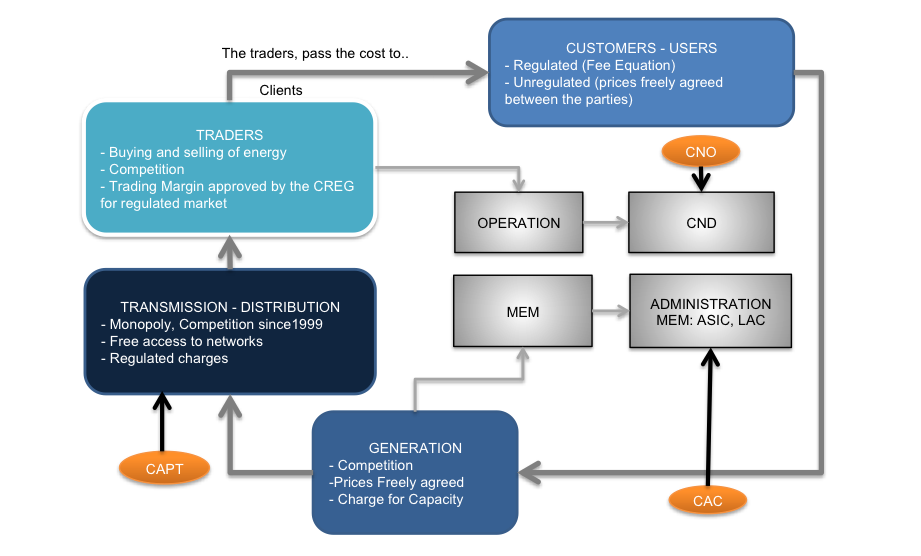
\includegraphics{fig1}  
\caption{Operational structure of the electricity market}
\scriptsize 
\textbf{Source: Comisi\'on de Regulaci\'on de Energ\'ia y Gas  (CREG)}
\captionsetup{justification=centering,margin=0cm}
\label{Fig 1}
\end{figure}

Where, 
\begin{itemize}	
\item 
\textbf{ASIC:} Administrador del Sistema de Intercambios Comerciales.	
\item 
\textbf{CND:} Centro Nacional de Despacho.	
\item 
\textbf{CNO:} Centro Nacional de Operaci\'on.	
\item \textbf{CAC:} Comit\'e Asesor de Comercializaci\'on.	
\item \textbf{CAPT:} Liquidador y Administrador de Cuentas del STN.
\item \textbf{LAC:} Administrador del Sistema de Intercambios Comerciales.	
\item 
\textbf{MEM:} Mercado de Energ\'ia Mayorista .

\end{itemize}

Since the enactment of laws 142 and 143 of 1994, Colombia has advanced to a process that aims to achieve efficiency in the provision of services derived energy demand in terms of quality and competitiveness \cite{Aguilar2004} \cite{sandoval2004}. This allows the presence of the liberalization of the market between agents generators and traders with the aim of ensuring transparency in price formation, while the transmission is constituted as a regulated monopoly that later became in an oligopoly.

The creation of MEM ``Mercado de Energ\'ia Mayorista", the subsequent establishment of the Colombian Energy Exchange in 1995 \cite{Aguilar2004}, creating ``Derivex" (for derivatives trading) and establishment of the Central Chamber of counterparty risk for compliance with leveraged transactions, seek the proper functioning of the energy market, where all participants act on an equal footing and under strict quality standards allowing free competition.

The basis for market functioning and creation of Colombian Energy Exchange, where the State established the right conditions for the generation and procurement guidelines for energy on spot markets, forward markets and contracts, began his term in 1995, through the resolutions CREG 24 of 1995 and 25 of 1995. Henceforth all regulatory changes have been referred to these resolutions so that the regulation of the operation of the system have been based on the same fundamentals. Nevertheless all the components of the framework do not consider the problems derivative of dishonoring the business commitments acquired between agents.

In other words, the regulation law defines the need for intervention in energy prices even in reservoirs when water levels are lower to higher operating minimal (decrease in supply). In this aspect, the charge for capacity was created because of the consideration to the guarantee of generation capacity (supply securing), among others, but again it refers from operational perspective, because the weather and rains are variables with high impact and difficult to predict, instead financial conditions can change in specific times according to the law, but it is not necessarily true.

Then, the classification between cogeneration, low generators and self - generators was the answer to the specialization of the system in the main activity (generation), establishing limits required for bids on the stock market as long as its generating capacity was superior to 20 MW and ensuring that market making is recurrent without discontinuity in the prices formation, it means more operative controls and the absence of corporate controls.

The market organization, as mentioned above is designed in four main activities: the generation that is the production of electrical energy, activity that must be connected to STN; the second one is the transmission which is responsible for transporting energy through its own infrastructure (at or above 220 KV lines), third the distribution with similar activities only on a lower voltage (less than 220 KV) and finally trading, specifically geared to the purchase and sale of electricity.

In the trading activity, transactions may be through bilateral financial contracts, freely agree between the parties, or through ``Colombian Energy Exchange" transactions similar to the stock market where the price adjustment responds to movements between supply and demand.

In the figure \ref{Fig 2} we present the main components of the energy market considering state intervention, in turn some of its own market interactions between agents and the management and control entities are presented. At each level it becomes possible to identify the participants, being the CREG the agency responsible for the regulation and UPME responsible for planning. There is an entity designated for the operation of the system, and it is responsible for ensuring the operation and functionality of the market \cite{Aguilar2004} his name is XM ``Expertos en Mercados". 

\begin{figure}  
\centering    
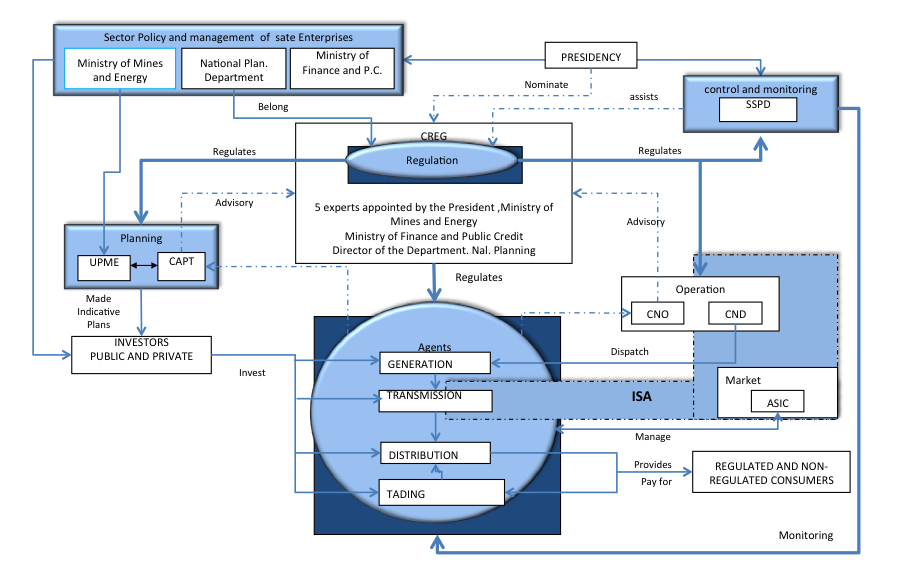
\includegraphics{fig2}  
\caption{Composition of the electricity market}  
\scriptsize 
\textbf{Source: Unidad de planeaci\'on minero energ\'etica (UPME)}
\captionsetup{justification=centering,margin=2cm}
\label{Fig 2}
\end{figure}

And thanks to the figure \ref{Fig 2} is it possible to identify that XM is the company responsible of the fulfillment of financial transactions, but is complicated take control of all financial decision inside of the agents.

\section{Operation of the electricity market} The electricity market consists of 5 major participants: generators, transmitters, distributors, traders and consumers, which are described below \cite{Aguilar2004}:

\subsection{Generators}are companies that produce energy, which can be traded on the Colombian Energy Exchange or through bilateral contracts. Installed capacity greater than or equal to 20 MW and different generation of edge of water (hydro) must submit offers of energy daily, valued at the price that forms per kilowatt / hour, in parallel must declare the availability of generation in order to program the dispatches.
\subsection{Transmitters}These companies record their income through remuneration indexed to some economic index, and the remuneration doesn?t depend of the used of the infrastructure (continuous flow of energy, congestion, etc.). This remuneration is done by calculating a new replacement value of network assets (present value discounted at a capital cost) and evolves depending on PPI (producer price index) nominal for the previous fiscal year. Simply the income is fixed and acknowledged from the availability of transmission assets and the possibility of their use.
\subsection{Distributors}These are companies whose business is also concentrated in the transportation of energy, but in voltage levels below 220 KW, allowing them to attend other lower voltage systems. These systems are divided into two: ``sistemas de transmisi\'on regional" (STR) and ``sistemas de distribuci\'on local" (SDL), and distributors are responsible for providing services to one or more trading markets.
\subsection{Traders}Are agents intermediaries who make an intermediation business, interacting with claimants of energy, generators, transmitters and distributors. They can operate in response to the regulated market (consumption of less than 0.1 MW), not regulated or even both. It is a treasury management business whose operation is similar to an investment fund. Risk exposures concentrated issues like financial affairs, credit, liquidity evaluations, market and operational situations, and all conditions must be given for carried out the dispatch of energy.
\subsection{Consumers}In the same way that the materials, consumers close the cycle thanks to his demand position of the energy produced. They are legal entities or individuals who require this product to ensure operation or just for everyday activities, thus the consumer determines the fluctuations in supply according to the behavior of the economy.

The operator of the energy market in Colombia has under its administration the functions of ``Centro Nacional de Despacho'' (CND), to manage the ``Sistema de Intercambios Comerciales" (ASIC) aand finally establish and manage accounts usage of charges in national networks (ASIC). The representation can be seen in figure \ref{Fig 3}. Similarly, the planning of the operation and the direct relationship with the agents, are crucial for the fulfillment of transactions. The operator evaluates the minimum levels of liquidity, solvency, capital and other financial conditions, for agents in order to participate in the operation in an equitable manner without compromising the supply, but the situation in the accounts of agents is out of control because of that the complete information is published each 3 months.
\begin{figure}  
\centering    
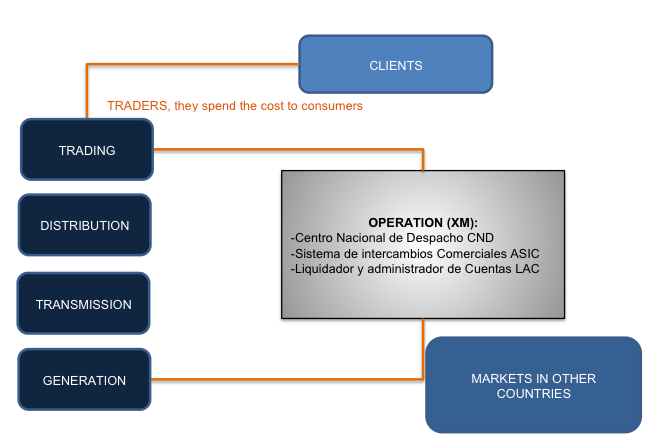
\includegraphics{fig3}  
\caption{Functions of the electricity market operator}  
\scriptsize 
\textbf{Source: XM}
\captionsetup{justification=centering,margin=2cm}
\label{Fig 3}
\end{figure}

One of the necessary conditions for ensuring energy supplies, wants to avoid the concentration of activities in the energy market, namely the generation, transmission, distribution and trading. Regarding generation (installed capacity), no company can own more than 25\% of total available generation in the country, which ensures the energy production function as a diversified portfolio despite the fact of large hydro exhibition that has Colombia. Likewise, a similar percentage for the trading and distribution activities (no more than 25\%) and the percentage extend through figures like equity method and indirect ownership (business castling) \cite{sandoval2004}.

The calculation of commercial offers is performed from the methodology of asset allocation using a tool for financial market management \cite{kuznetsova2014}. All participants must provide financial guarantees as required by the regulation and in the case of generators and traders, exists a direct request to participate in energy exchange. Thus, each participant agent has a number of rights and obligations to be met fully, with the final purpose of ensured the power supply and avoiding risks that could pose a high severity.

A specific case that concerns to the planning central of energy has to do with the re-dispatch, which refers to the rescheduling of initial supply. If there are operational deviations around 5\% (VaR at 95\% of confidence) on the generation of programmed energy, will lead to penalties for generators that will be paid in cash and the settlement is established considering the spot energy price and the price of offer that the generator present when they make the reprogramming  \cite{sandoval2004}. 

This is a sample of intervention by the operator, and in the case of financial exposure, nowadays the legislation considers the capital capacity but not the materialization of systemic risk generated by the interactions.

The above is a specific case of risks, and necessarily will be considered when all exposures of the agents should be integrated, also when investigations identified what are the best ways to relation the variables in a global context of risks. In any case, the representations of integral physical phenomena but in this project the consideration of financial branch.

\section{�Why it is a complex system?} A system is a combination of different logical or even physical entities that interact with each other to establish a specific purpose, namely to reach a target from the relationship between them \cite{sole2009}. The systems can be dynamic, and it means that the behavior changes over time, or the systems can be stable, where the conditions, generally do not change and remains in equilibrium \cite{boccara2010}.

The complexity meanwhile, as defined by \cite{sole2009} can be understood as the level of difficulty with which we can predict the behavior of a variable or an overall system, thanks to its internal characteristics and their relationship with the environment.

Similarly after setting the behavior of those variables or systems, with the respective interactions, it is possible to determine that behaviors can be simple if the complex origins are clearly identified.

Complex systems for their part, are composite systems with many parts (or variables), with many degrees of freedom that are not equivalent between them \cite{levy1994}\cite{tumminello2005} meaning that each element is independent in making their decisions and governed by different parameters \cite{tumminello2005}. That said we could define complexity as the study to determine how complex systems can generate simple behaviors \cite{sole2009} but only if the origin of complex situations is understood, in other words if the physical phenomena are completely comprehended.

A physical phenomenon according to the chemical theory, are those transformations in a body that does not change the nature of matter of which this is constructed, for example, rain, wind, electric power transformation in motion \cite{stavridou1989}. And these phenomena can be transferred to other sciences, such as economic phenomena that are associated with the activities of individuals seeking the transaction of goods or services. 

At the same time, there are countless examples that can be categorized as a complex system, within which stands out: The operation of a vehicle, with many independent components related and how they make the movement rolling in the street; a swarm of bees where each participant has defined functions and all of them seeking survival; or even one complex system could be the life itself \cite{tesfatsion2003}\cite{tumminello2005}. The human body has different physical components that seek the survival of the organism, if a component fails, the system could collapse.

Ants, for example as shown in figure \ref{Fig 4}, have a complex behavior because each member performs activities defined by natural selection \cite{boccara2010} and do not require a central control to ensure the functioning of the system (the ant colony), it means the queen let each member do the job. In addition to the above, such systems benefits from the self-learning as a defense mechanism against possible future instability.

\begin{figure}  
\centering    
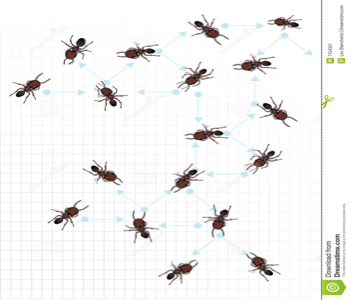
\includegraphics{fig4}  
\caption{Ant behavior} 
\scriptsize 
\textbf{Source: es.dreamstime.com}
\captionsetup{justification=centering,margin=2cm} 
\label{Fig 4}
\end{figure}

A company is by definition a complex system as it is composed of different elements, such as fixed assets, intangible assets, employees, customers, suppliers, investments, intellectual capital, shareholders, among others.

Each of these elements is integrated together to perform a complete and complex function, which turns out to be the financial viability of the company and its sustainability \cite{yang2015}. 

Similarly, if one of the elements of the business fails, then the stability of the system is compromised and hence its future functionality, namely if in certain case of affectation in the productive assets, clearly there would affect the core business.

In line with the above, if a company seen like a unit can be classified as a complex system, a group of companies that interact with each other also will be. Such is the case of trade markets where transactions determine the degree of relationship between the participants \cite{jiang2014}, which therefore seek the sustainability of the system in the long term, ensuring their preservation and profitability. 

If one of the elements of the system presents problems for continuity, viability is compromised to a great or lesser degree depending on the relative size of the affected agent.

By comparison, if a trade market is a complex system, it is more difficult to estimate the generation of profits consolidated compared with the estimate of profits for a specific company. However, from this research project it is possible approximate the interactions between participants and the dynamics of their profits to integrate them later from the perspective of complex dynamics  \cite{boccara2010}\cite{levy1994}, allowing approach from the actual view to economic viability of the whole system, involving financial risk susceptibility from agents.

Since the liberalization of international markets with globalization and access to information, it is necessary ensure the operation of enterprises in competitive environments, independent if its role is as a production company, service provider, public or private. Thus, control of its financial performance makes them to assimilate evolving global challenges, and allowing interaction with the environments to become a dynamic system \cite{jiang2014}\cite{yang2015} \cite{Wyman2011}.

As we mentioned, to determine the level of profitability from the systems, it is easier to measure individually instead of collectively. However, there are studies where is more useful make a measurement of returns integrated and then reduce it to the individual level, in this sense applied research on credit risk using dynamic complexity can taste this relationship\cite{jiang2014}\cite{yang2015} . 

The results found in \cite{yang2015} create a scenario for future research on financial problems, economic and risk, where it is possible to understand the complexity of their individual results on the overall performance.

\section{Models used for measuring market performance}The inclusion of processors to perform calculations from the decade of the 60's was of vital importance to achieve results in record time from simulation processes and iteration. The XXI century came with important advances from mathematics that purported to describe the operation of physical phenomena giving space to strong research and development \cite{kwapien2012}.

Among the advances, game theory began as a methodology that sought to respond to the economic phenomena of interaction between participants in a system \cite{lebaron2005}. 

The first studies were concentrated on describing mathematically as the process of decisions, evolves in perfect environments of knowledge among participants of the process \cite{medina2007}. In turn, further research evolved into a complex mathematical language, giving way to new definitions of philosophy that openly exceeded the initial proposals.

Moreover, agent based modeling (ABM) emerged as a promising method to advance the understanding of the systems under dynamic conditions \cite{fischer2014}. The inclusion of that methodology allowed the evolution of each element and level of impact through integrated models, achieving easily understand operation for management and control resulting from the integration of the components using equations.

Indeed, electricity markets are experiencing a number of constraints and uncertainties when executing investments because of the situation of weather and climatic changes. Each decision maker is autonomous, and requires preliminary information that incorporates the ability of agents to interact, communicate and negotiate with each other. The agent based modeling provides this possibility \cite{gnansounou2004} and also to simulate individual situations that enrich the analysis.

The agents are autonomous, distributed in a system and are ``intelligent", i.e. that they are communicative, rational, adaptive and they learn \cite{gnansounou2004}, characteristics which becomes in the main contribution of agent-based modeling.

Similarly, the complexity helps to establish more structural way each of the taken decisions considering the inclusion of chaotic behavior and the butterfly effect \cite{costa2007}. TThe complexity comes in a system consisting of interrelated parts, which together generate results not so evident \cite{costa2007}. 

Complex systems usually are not as complicated systems, because his intention is to be a simple explanation of physical phenomena; in this regard we can analyze and find the elements that produce complex behaviors.

And finally, one of the great contributions of the complex dynamics is that we can define mathematically the interactions among participants, the type of operations that have each other, and the kind of relationship useful for determine through equations of first and second degree the level of complexity \cite{costa2007} \cite{newman2003}. Thus physical phenomena are reduced to mathematical expressions in sets of soluble real numbers.

\subsection{Game Theory} Game theory was born as a mathematical methodology applied initially in problems with economic nature and is based on strategies that are taken from what is estimated will be the decisions of others  \cite{gibbons1997}. Each participant in the process has access to certain information, which will allow managing the risks and how they will take their decisions.

A game is a mathematical representation that includes strategies, actions, number of participants (these may be individuals or organizations), probabilities and profitability \cite{neumann1947}. Thus there is an interdependence that involves each of the players (agents) in the decision process and the decisions that they take will affect others. 

The combination of strategies to improve the profits of the participants, will be understood as a equilibrium in the game, although it will be static while initial conditions do not change \cite{agarwal2012}, in this sense it is important to note that static condition is one of the biggest problems of game theory, given that the initial conditions of the systems are evolving constantly.

Similarly, the modeling of the electricity market as a game searches to achieve results maximizing profits for each of the participants considering initial conditions. A further problem is that this approach assumes a thorough understanding of the characteristics of each participant and from a financial point of view is difficult to establish the planning of all system elements.

The elements of a game are \cite{gibbons1997}:

\begin{itemize}	
\item 
\textbf{Players (N):} individuals who have to make decisions, always assuming that seek to maximize their utility, in the case of energy markets, the agents.
\item \textbf{Actions (X):} Possible alternatives that a player can take at any moment where you should decide, e.g. buying and selling decisions in the electricity market.	
\item \textbf{Information:} Degree of knowledge that is available at all times for everyone, about the values that take different variables and status of other participants.	
\item \textbf{Payoffs (U):} represents the value received by players at the end of the game as a profit, in this case the net profit after interest for electricity market agents.	
\item \textbf{Equilibrium:} set of strategies that players take for play the game, searching the optimizing the payoff function (profit) in front of others. \cite{neuhoff2005}
\end{itemize}
The mathematical expression of a game is presented as follows \cite{cachon2004}\cite{gibbons1997}:

\[G = [N, X_i, U_i] \quad \forall \, i = 1, 2, 3, ..., n\]Players: $N = 1, 2, 3, ..., n $ is a finite set of~$n$, indexed by~$i$.
Set of actions for the player $i$ $x_i$

$x_i$ = ($x_1$, $x_2$, ..., $x_n$) in the case of electricity market, this set consider purchases and sales of energy, defined in quantity of energy traded (i.e. kwh).

Utility function or ``payoff" for player $i$: $U_i$

$U_i$ = ($u_1$, $u_2$, ..., $u_n$) is a profile or functions of utility \cite{gibbons1997} \cite{tushar2013}

The most important assumptions of game theory, according to, \cite{li2013} are:

\begin{itemize}	
\item All agents are interested in their own ambitions.
\item Each agent has a utility function.
\item The preferences of each agent can be described by the utility function.
\item Every agent knows the possible actions taken by the others.
\end{itemize}
From the foregoing, game theory is emerging as a useful tool for describing various phenomena in the markets, despite the fact that the assumptions for their implementation are quite idealists. On this basis it is possible to define strategies in different environments that enable it to be the best response to competitors giving way to the calculation of the equilibrium, which speaks of profits in competitive environments and is the best strategy on the part of the participants [ME].

\subsubsection{Nash Equilibrium} It is possible calculate it, in environments of perfect competition, but the final decisions do not consider the likely reactions of rivals \cite{gatti2013} \cite{gibbons1997}. This because such decisions associated with any of the participants will have a negligible impact on market behavior that can be discriminated. The most important task of the participants is to anticipate market behavior and how to maximize profits \cite{stoft2002}.

That said, the measurement proposed by ``Cournot" in his competition model \cite{day2002} \cite{dekel2014} \cite{tushar2013} can be adapted, because for the electricity market in the first phase, companies compete for power capacity that can be produced, while in the second phase, companies compete for the amount of energy that they can trade.

In the Nash equilibrium each participant knows which is his best strategy taken, and all participants known the strategies of others \cite{day2002}. It can also be understood as a harmony in which a change of strategy does not put the agent in a position of advantage over their profits \cite{gibbons1997}. 
The main problem is that for achieve the equilibrium does not exist simple calculation tools when there are a large number of agents with different strategies.

The electricity market, therefore, operates as an oligopoly considering the generation process because in Colombia there are few big generators, and some strategies are previously known in the business chain.

For example, the producer will maximize their profits by producing more energy than usual in the absence of climatic, operational or external events, although subject to restrictions by the regulator of the system, associated with the installed capacity and the satisfaction of demand.

Traders know the strategy who was chosen by generators and they make purchases of energy through bilateral contracts in order to hedge against the existing volatility in demand and inside of the creation of prices, in turn such decisions are being evaluated considering local and international economic conditions.

The prisoner's dilemma is an example \cite{alos2003}\cite{buttler2013}\cite{gibbons1997} which runs between agents descriptively but only for two participants. However, the Nash equilibrium occurs when traders, consumers and power generators that are part of the global market, have adequate energy exchanges, so that the returns and profits are under acceptable levels of risk aversion, but this is not so obvious as a final solution.

Mathematically, Nash equilibrium can be defined as follows: \cite{gibbons1997}\cite{von2009}:
If each agent knows what everyone else will go to do, it would be easy to pick his own action and in this terms optimize his profitability function, i.e. the player (agent) does not have arguments for change the strategy  \cite{von2009}.

With,
\[U_i = (u_1, u_2, ..., u_n)\]
And also,
\[x = (x_i, x_{-i})\]
Then,
\[U_i(x^*_i, x^*_{-i}) \geq U_i(x_i, x^*_{-i}) \quad \forall \, x_i \in X_i\]
This means that $x^*$ is the best response that is the best strategy against competitors or agents to maximize their profits.

\subsection{Agent-based Modeling}

For many years the research question posed from different areas of science, focused on how to describe the characteristics of participants in a system and their relationships \cite{yao2008}. Agent-based modeling (ABM) has become a useful tool to approach the complexity of the interactions between the elements of the systems and the methodology has begun discussions about the degree of difficulty with which each system should be treated with their respective peculiarities.

However, describe phenomena that explain the relationship between the agents through equations is quite complex \cite{zhou2007}, i.e. it is not a simple process because the consideration of all characteristics through a single mathematical expression in a linear or polynomial way can be sometimes a simplistic explanation of physical phenomena. 

Similarly evolutionary systems with self-learning, independents, with high or low dynamic, among other things, are collecting certain relationship that is not easy to interpret \cite{newman2003}.

The financial and economic field is no stranger to the phenomenon, as it considers certain characteristics typical of ABM. That was how, in the early twentieth century when models like the CAPM for the allocation of capital assets, the model Sharp for determining optimal portfolios, the ``Black - Scholes" model which applied stochastic concepts on financial options and overall classical financial theory derived of concepts of Alfred Marshall \cite{humphrey2004}, among others. They were nothing more than the results of consider the relations between elements present in the markets through equations.

In that way, there are many components considered about the description of the physical phenomenon (equations). For this reason, the reliability of the estimates has been compromised for long time. Such is the case of the success of the "Black Scholes" model for option pricing in the early 90's and the subsequent bankruptcy of the investment fund managed by their creators \cite{greenspan2007}.

This, because at the end, the results of the equations may partially explain the phenomenon or not, and the explanations of the failures is they do not consider all the variables involved. Then, the theoretical frameworks started to talk about heterogeneous subsystems, and those advances makes the descriptions and further analysis are critical and more adjusted \cite{kuznetsova2014}.

An example that sums up this phenomenon is the hypothesis of efficient markets proposed by Eugene Fama in the 60's. In the theory, the behavior of financial markets is simplified through the ability to predict future prices using one equation with different assumptions \cite{malkiel1970}:

\[Y_t = \mu_t + \epsilon \]

This formula is a reduction of phenomena occurring around predictions of future prices. However, the ``random walk" continues being a relevant theory as a starting point for assumptions and simulations of financial process. While the expression is quite simple at least in mathematical terms, today remains a benchmark for understanding the mechanics of the agents crossing transactional information in the financial markets, even though many of the assumptions are difficult to fulfilled.

The Figure  \ref{Fig 5} present a generic evolution that can be estimated from historical data stored, however there are a lot of variables involved in the forecasting process that are not considered.

\begin{figure}  
\centering    
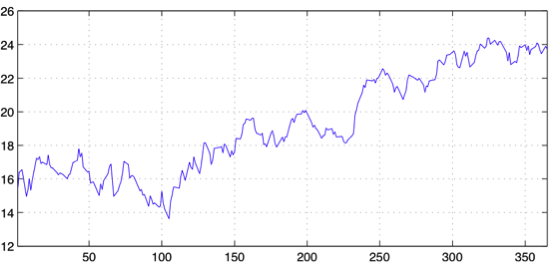
\includegraphics{fig5}  
\caption{Random Walk example}  
\scriptsize 
\textbf{Source: Own calculations}
\captionsetup{justification=centering,margin=2cm} 
\label{Fig 5}
\end{figure}

Continuing with the task of explaining the physical phenomena using formulas, if each of the agents involved in the financial market (investors, issuers, regulators, intermediaries, etc.) has similar behavior, described by the equation of random motion, then the aggregation of each of these behaviors could yield comprehensive income around the market, nevertheless, model the behavior of the participants by means of equations, is not an obvious process.

\subsection{Complex Systems}
In a beehive, whose functionality is subject to the work performed by each individual, it can be prove that the total of the members performed their role in certain tasks considering their condition. 

It means that bees are classified naturally. Gordon \cite{boccara2010} pointed out for example, that for ant colonies the assignment of tasks is a continuously adjusted process, in other words, independent of the role executed by each ant either physical work, military, procurement of food, cleaning, among others, all the distributions are reviewed periodically. 

Ants permanently adapt to the situation without having a supervisory figure to fulfill their duties. In other words there is no central control, the queen not decides who does \cite{boccara2010}, allowing the generation of a very proper emergent behavior of complex systems.

There are many examples of complex systems behavior, among which we can highlight the urban transport network, where each participant can be classified as a member of the system; a company, given the interactions among members of the organization and subsequent guidance to achieve the objectives \cite{levy1994}; the telecommunications systems, being interrelated through a data transmission network; the economy, thanks to the high need to consider a number of variables to maintain a nation under budgetary control; among others.

The definition of a complex system comes from different disciplines such as biology, ecology, game theory, philosophy and others, which historically have tried of modeling the relationship between each of the components of the systems, or agents and his subsequent integration through mathematical descriptions. The main features for existence of complexity in a system according to \cite{boccara2010}\cite{sole2009} are:

\begin{itemize}	
\item Existence of a large number of agents (individuals) that interact.
\item The self - organization of collective behavior, which makes difficult to anticipate the knowledge of the behavior of each agent in the future (state of emergency).
\item The emergent behavior is not the result of the existence of a central control, but rather of the self - learning.
\end{itemize}

The agents are then vital part of the systems, and they have different features among which stands out its ability to interact with one's environment and that they can respond to what happens around them despite the existence of a stated purpose or not \cite{boccara2010}\cite{sole2009} . 

A set of agents forms an organized population, for example in the case of bees, the hive is created and in the case of the existence of buyers and sellers the market is created. For purposes of this research, power generators, transmitters, distributors, traders and consumers are part of the energy market as a global system.

Subsequently, The populations organized in turn grouped all the learning from agents and their autonomy and the strategies that they taken as a way of responding to the environment, and if the strategies are aggressive or otherwise passive \cite{tumminello2005}, it means the self learning can improve the survivor of the system or let it fail.

As already mentioned, systems are a set of populations where agents applied their strategies \cite{boccara2010} using the tools that they have and amid external conditions. The complexity arises when there are many interrelationships between elements, so that the change in the strategies of the agents can affect the behavior of the system in the future.

In financial terms, a default of one of the agents involved in the energy market transactions, can trigger problems in the system, thanks to transactions that they have between them, increasing the probability for demand will be unattended.

In the literature, it is possible to find two classifications for systems, if they contain populations seeking to adapt to the environment are called complex adaptive systems, but when several populations of agents adapt to each other the result is a system co - evolutionary, and the system self-learns from experience \cite{boccara2010}\cite{sole2009}\cite{tumminello2005} iIt means improve the performance considering the evolution. 

In the case of electricity markets, thanks to the operation itself, each population group (traders, generators, transmitters, consumers) performs the same activities and evolves based on the optimization of its results, referring to maximize profits but at the same time reaching the minimization of the total risk.

There are three elements required to understand the complexity, which are: variation, interaction and selection. Variation is the main component of the adaptation of the system given that it is necessary to find a balance between uniformity and differentiation (variation) so as to make easier propose solutions to those agents that do not conform to the average in your behavior \cite{boccara2010}.

On the other hand, interaction refers to the elements related, when and how, under the conditions set. This interaction is not always symmetrical, much less uniform; it can be very intense (high relationship) or diffuse (low relationship)  \cite{sole2009}\cite{tumminello2005}. It is clear that for electricity market agents, interactions are present thanks to the cash flows exchanged between them considering purchases and sales of energy. 

In this sense, it will be intense interactions when flows will be high, where the amount of contracted energy is large (large number of bilateral contracts) and will be diffuse when the amount of energy exchange be low or non existent, it means when they doesn't have business each other.

The third element is the selection, which refers to agents which should be replicated and which should be eliminated \cite{boccara2010} not only through the process of natural selection but rather because of the qualities that can transmit to other agents, using decision criteria that are concentrated in cost, time, benefits, among others, or for the purposes of this research project, the risk level.

From the point of view of financial risk, an agent that sees their income statements compromised can incur in events of default and maybe it can't honor their commitments, subsequently affecting other agents for non-payment. This project proposes the identification in advance of such event risk with the aim of reducing problems in the operation of the market, and ensures the financial functioning of the system.

The figure \ref{Fig 6} shows a vectorial behavior regarding diversity of agents involved in the system, the result after the processes of variation, selection and interaction converge to equilibrium considering initial operating conditions.

\begin{figure}  
\centering    
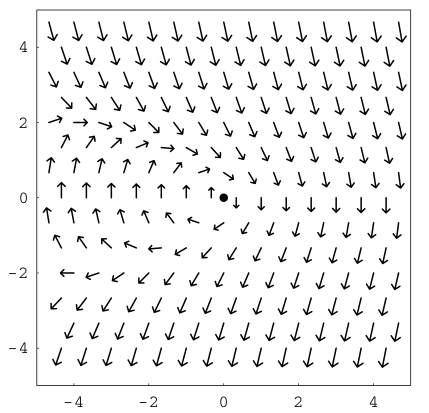
\includegraphics{fig6}  
\caption{Convergence in 2 dimensions}
\scriptsize 
\textbf{Source: Nino Boccara }
\captionsetup{justification=centering,margin=2cm}   
\label{Fig 6}
\end{figure}

It is important to talk about models that describe the complexity mentioned above, and for such purposes the mathematical tools proposed by \cite{boccara2010}\cite{tumminello2005}. are a solution to this problem. Although there are a number of essential elements in each system, this does not ensure that under the mathematical rules are necessarily considered. They should contemplate only the factors those needed to describe and understand the physical phenomenon. 
Models must be sufficiently complex to capture all the relevant characteristics, but also, simples considering only key issues.

On the other hand, a dynamic system begins to respond to questions about how to relate to the participants and the particularities [38]. Physical phenomena can be described by equations where each solution is determined by the initial conditions fed into the system, resulting relationships between agents. For its part, the description of evolution, its adaptability, the factors necessary for the administration and decision-making will be results of the complexity level for describe the phenomena \cite{tesfatsion2003}.

Therefore, the electricity market considers, many of the characteristics of complex dynamic. It means, the interactions between agents, self-learning, the selection of the best-positioned participant and the ability to adapt to evolving environment. Those characteristics are crucial to the formation of prices and ensuring energy supply, as long as no commitment of system operation. In other words and for the purposes of this research project, the system is stable, if financial risks are not present.

\subsubsection{Chaos}

A negotiation process where different actors are involved, which seek to maximize their profits (or particular interests), is an example of deterministic evolution when we have no more information than what is intended to negotiate \cite{newman2003}. Such interpretations for many years were the center of the studies until the early twentieth century when the study of phenomena, wanted to predict with certainty the evolution with more variables integrated \cite{levy1994}.

Poincar\'e [35] in their previous studies, established that the variables involved in the decision process, could develop a chaotic behavior observable through evolution. Thus, takes place the birth of chaos as a differentiator for all the analysis that attempts to predict with certainty the evolution of each system. Chaos does not mean simply disorder, chaos is simply a different order, which must be analyzed in another way \cite{levy1994}.

It is possible to classify the phenomena according to their level of complexity and adding an additional element as the chaos (unpredictable component), but does not mean that behaviors tend to be random, chaos means that they have an underlying evolutionary order, always determinable, and when we know the initial conditions \cite{levy1994}\cite{sole2009}.

Then, by varying initial conditions, for real systems we can have very significant effects, all of this in front to small changes, which generate cascade effect or strong impact with high severity \cite{kwapien2012}. 

An example of this can be the change in the regulation of electricity markets, specifically capital requirements, e.g. a company that does not have this requirement can pass to be insolvent and generate serious financial consequences. The chaos is deterministic because there is some factor, or some component that determines their behavior \cite{levy1994}\cite{tesfatsion2003}.

Chaos theory has been misinterpreted because the first description is the existence of apparently disordered systems, but actually what it claims chaos theory is finding the underlying order in data apparently random \cite{levy1994}. 

For purposes of this research, chaos represents a scenario, where the electrical system exhibits difficulties from the financial point of view, considering that one of agents doesn't have the capacity to respond to its commitments. That is, the generation of ``default" situation (nonpayment) that implies the affectation of supply levels according to small changes in initial conditions.

And initial conditions are the stability at the beginning of the process, the organization of transfers and the accomplishment of the financial conditions for operate the market as a trader.

\textit{``If a butterfly stirs up the air in Beijing, it can change the storms system in New York next month"} (Gleick).

\subsection{Advantages}

Many studies have focused on defining the energy demand levels in the medium and long term over energy systems and their administration \cite{medina2007}\cite{sweeting2007}\cite{weidlich2008}, in order to ensure the supply level. The optimization process meanwhile, reproduces such models to integrate the elements and achieve high standards of performance at low costs. Growth is evident, between 1980 and 2005 the level of demand of fuel for power generation (in Mboe) grew nearly 60\% \cite{sweeting2007}, giving sufficient bases for studying this subject.

Planning the performance of the energy system is not an easy task, and therefore is necessary dispose of tools to achieve this goal, starting from classical macroeconomic models unto the more integrated models.

The purpose of this work is to do planning of energy dispatched but considering optimal financial systems, and the results must evaluate the agents in terms of financial risk. And there are an additional goal related to the ability to predict the presence of negative events associated with the risk indicators.

In turn, the creation of useful tools to ensure commercial exchange and the energy supply, it provides innovative elements of analysis in business decisions. Similarly generating functional components who seek the sustainability of stakeholders (central operators and trader agents) from the point of view of profitability and sustainability.

This task requires of a series of conditions of economic nature, technical and of resource availability, being some areas such as power generation capacity, minimization of generation costs, minimization the consumption of conventional resources and the equilibrium between supply and demand \cite{weidlich2008}\cite{wolfram1999} those requires special attention because they implicitly must be integrated into the results.

Historically there are some models that have been implemented with quite results interesting for the planning of the operation, which are responsible for identifying as the price or availability of energy affects the general economy \cite{jackson2010}\cite{krause2006}\cite{weidlich2008} with based on the impact on its gross domestic product (GDP), unemployment, inflation, the producer price index, exchange rate, among others, and vice versa.

The great advantage of these historical models is their ease of implementation based on historical data and seasonality of the series. The proposal with this project is to have a tool with more component that can be integrated with the previous developments.
However, as was mentioned throughout the chapter, studies have focused on determining operational and even general expositions, by measuring the economic impact severity of operating events internal or external.

Finally, the breakthrough that suggests this work, is the possibility of study directly the financial phenomenon implicit in the operations, and synchronize with operational and macroeconomic developments that results in more robust models for analysis, i.e. integrated.

Thus, with a identification of interactions and impacts, we can avoid affecting the system sustainability, by managing a new branch of financial innovation, which is called systemic risk very different from conventionally known systematic risk.


\bibliography {Biblio}
\bibliographystyle{plain}



\end{document}